\documentclass{beamer}

\usepackage[utf8]{inputenc} % Включаем поддержку UTF8  
\usepackage[russian]{babel} % Включаем пакет для поддержки русского языка 

\title[Spherical Principal Component Analysis]{Spherical Principal Component Analysis}

\subtitle{Applying spherical PCA algorithm for dimensionality reduction set of unit vectors}

\author[] { Белоусов Илларион, Курбет Игорь, Малашенко Сергей, Машинсон Всеволод, Свиридов Илья }

\date[]{OZON Masters, December 2020}

\begin{document}

\frame{\titlepage}

\begin{frame}
\frametitle{Постановка задачи}
\begin{itemize}
 \item В задачах классификации и распознавания объектов хорошо себе зарекомендовали модели, которые оценивают близость 
 $$X_i \in S^n = \{ x \in \mathbb{R}^{n+1} : \left\lVert x \right\rVert=1 \}$$
 \item В работе предлагается снизить размерность $n$ при помощи метода гравных компонент на сфере $S^n \Rightarrow S^m$, где $m < n$.
 \item Качество алгоритма оценивается решением задачи кластеризации векторов $X_i \in S^n, \tilde{X_i} \in S^m$ в предположении, что $$X_i \sim \sum_{i=1}^{N}\pi_i \mathbb{V}_{n+1}(x | \mu_i, \kappa_i), \mathbb{V}_d(x | \mu_i, \kappa_i)=\frac{\kappa^{\frac{d}{2}-1}}{(2\pi)^{\frac{d}{2}}J_{\frac{d}{2}-1}(\kappa)} e^{\kappa \mu^{\top} x}$$
\end{itemize}
\end{frame}

\begin{frame}
\frametitle{Решение задачи}
Решение общей задачи разбивается на три подзадачи
\begin{itemize}
 \item Разработка и сравнение моделей классификации на наборе данных MNIST. Модели строятся с использованием $SoftMax + NLL$, и $ArcFace$. Для функции потерь $ArcFace$ результатом будет совокупность $X_i$ на тестовой выборке
\item Разработка инструмента, который реализует метод главных компонент на сфере $X_i \in S^n, \tilde{X_i} \in S^m$
\item Разработка инструмента, который решает задачу кластеризации векторов на сфере
\end{itemize}

\end{frame}

\begin{frame}
\frametitle{Модель классификации}
\includegraphics[scale=0.3]{mnist_model.png}
\includegraphics[scale=0.3]{mnist_vgg8_3d.png}
\includegraphics[scale=0.3]{mnist_vgg8_arcface_3d.png}
\end{frame}

\begin{frame}
\frametitle{Метод главных компонент на сфере}
\begin{centering}
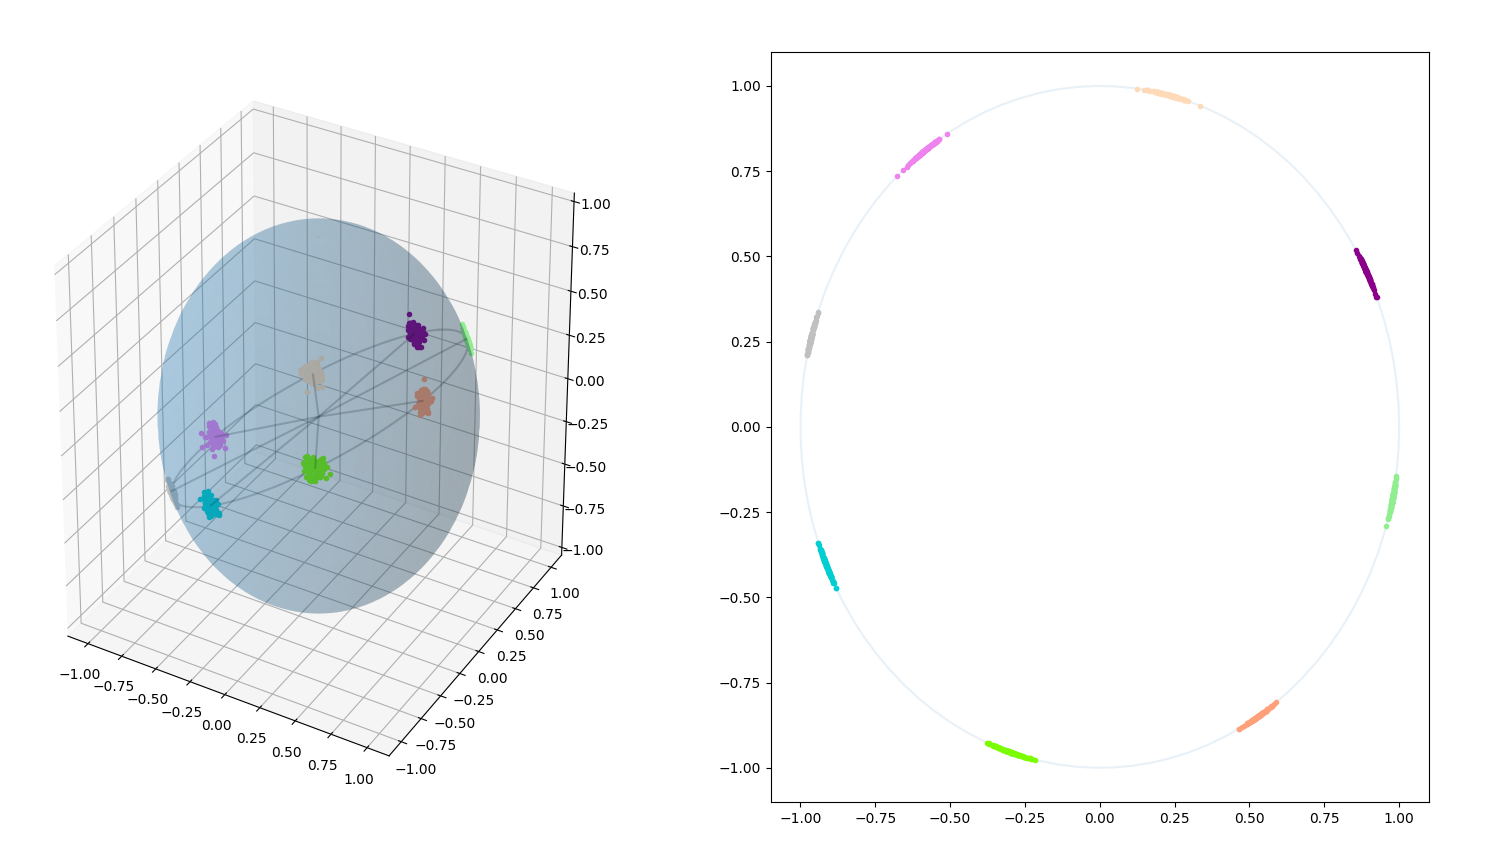
\includegraphics[scale=0.17]{sphericalPCA.png}
\end{centering}

$$\underset{\mathrm{U} \in \mathbb{R}^{m x r}, \mathrm{V} \in \mathbb{R}^{r x n} }{minimize} \lVert \mathrm{X - UV} \rVert^2_F, \mathrm{U} \in \mathbb{U}, \mathrm{V} \in \mathbb{V}$$
$$\mathbb{U} = \{\mathrm{U : U^{\top}U=I }\}, \mathbb{V} = \{ \lVert \mathrm{v_j} \rVert = 1, \forall j \}$$
\end{frame}

\begin{frame}[t]
\frametitle{Метод главных компонент на сфере}
\begin{align*} 
\mathrm{U(k+1)} &= \underset{\mathrm{U} \in \mathbb{U} }{argmin}{\lVert \mathrm{X - UV(k)} \rVert^2_F} \\ 
\mathrm{v_j(k+1)} &= \underset{\lVert \mathrm{v_j} \rVert = 1}{argmin}{\lVert \mathrm{x_j - U(k+1)v_j(k)} \rVert^2_2, \forall j}
\end{align*}
$$\Downarrow$$
\begin{align*} 
\mathrm{h(U,V)} &= \lVert \mathrm{X - UV} \rVert^2_F = \sum_{j=1}^n \lVert \mathrm{x_j - Uv_j} \rVert^2 \\
\mathrm{U(k+1)} &= \underset{\mathrm{U} \in \mathbb{U} }{argmin}{ \langle \mathrm{U-U(k), \nabla_Uh(U(k),V(k))} \rangle + \frac{\mu}{2} \lVert \mathrm{U - U(k)} \rVert^2_F } \\ 
\mathrm{v_j(k+1)} &= \underset{\lVert \mathrm{v_j} \rVert = 1}{argmin}{\lVert \mathrm{x_j - U(k+1)v_j(k)} \rVert^2_2, \forall j}
\end{align*}


\end{frame}

\begin{frame}
\frametitle{Кластеризация данных на сфере}

\end{frame}

\begin{frame}
\frametitle{Выводы}
\begin{itemize}
\item Использование нормированных векторов в задачах классификации и распознавания, позволяет повысить качество работы модели.
\item Метод главных компонент на сфере позволяет снизить размерность результирующих векторов, что приводит к повышению локализации кластеров, а также повышению производительности работы общей системы.
\end{itemize}

\end{frame}

\begin{frame}
\frametitle{Выводы}

\end{frame}

\end{document}
